%%%%%%%%%%%%%%%%%%%%%%%%%%%%%%%%%%%
\section*{Markov chain Monte Carlo}
\begin{frame}{MCMC: The best bad method you have ever seen}
Markov chain Monte Carlo (MCMC) methods are a broad class of stochastic algorithms to compute integrals.

Suppose you are confronted with the following question: what is the ratio between the circumference of inscribed circle and its diameter?
You are \textbf{not} allowed to use any Geometry.
\begin{figure}
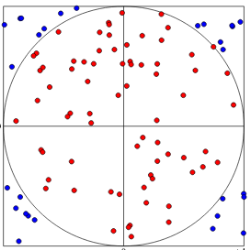
\includegraphics[scale=0.85]{figures/pi_MC.png}
\end{figure}
\end{frame}
%%%%%%%%%%%%%%%%%%%%%%%%%%%%%%%%%%%
\begin{frame}{First, a warning}
\begin{quote}
 ``Monte Carlo is an extremely bad method; it should be used only when all alternative methods are worse.''
\end{quote}
Alan Sokal (1955-) in \textit{Monte Carlo Methods in Statistical Mechanics: Foundations and New Algorithms} (1996, pg. 1).
\begin{figure}
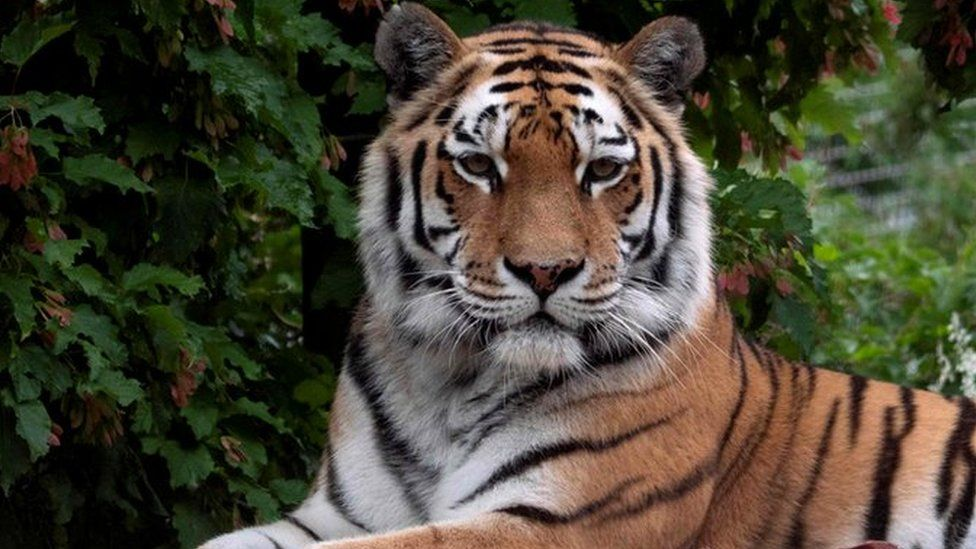
\includegraphics[scale=0.25]{figures/tiger.jpg}
\caption{MCMC is, in a way, like a captive tiger...}
\end{figure}
\end{frame}
%%%%%%%%%%%%%%%%%%%%%%%%%%%%%%%%%%%
\begin{frame}{Also...}
 Repeat after me,
 \begin{idea}[Bayesian MCMC is not a thing]
 \begin{center}
  {\Huge There is no such thing as ``Bayesian'' MCMC.}
 \end{center}  
  
  MCMC is a numerical method for computing integrals.
  It does not care whether you are a Bayesian, frequentist, \textit{flamenguista} or \textit{corintiana}.
 \end{idea}
\end{frame}
%%%%%%%%%%%%%%%%%%%%%%%%%%%%%%%%%%%
\begin{frame}{Computing integrals}
Technically, for a probability space $(X, \mathcal{F}, P)$, for $f : X \to \mathbb{R}$, we want to compute
$$
\mu_f = E_P[f] = \int_{X} f\,dP.  
$$
When $P$ is absolutely continuous with respect to the Lebesgue measure, we have 
$$
\mu_f= \int_{X} f(x)p(x)\,dx,
$$
as is usually written in introductory textbooks.

A ``natural'' approach to obtain an estimator of  $\mu_f$ is
$$
\hat{\mu}_{f, N}^{\text{MC}} = \frac{1}{N} \sum_{n = 1}^{N} f(x_{n}),
$$
with $x_1, \ldots, x_N \sim P$.
\end{frame}
%%%%%%%%%%%%%%%%%%%%%%%%%%%%%%%%%%%
\begin{frame}{A central (limit) theorem}
Define
$$
\text{MC-SE}_{N}[f]
= \sqrt{ \frac{ \text{Var}_{P}[f]}{N} }.
$$
Then
$$
\lim_{N \rightarrow \infty}
\frac{ \hat{\mu}_{f,N}^{\text{MC}} - \mathbb{E}_{P}[f] }
{ \text{MC-SE}_{N}[f] }
\sim \text{Normal}(0, 1),
$$
\begin{idea}[MCMC-CLT needs to hold]
 A key insight is that MCMC only trustworthy when a central limit theorem holds.
 This means $f$ needs to be $2+\epsilon$-integrable with respect to $P$.
 Look out for $\text{MC-SE}$, too. 
 It is important to quantify ``the probable error of the mean''\footnote{A ``pun'' with William Gosset's (1876--1937) paper: Student. (1908). The probable error of a mean. Biometrika, 1-25.}, as it were.
\end{idea}
\end{frame}
%%%%%%%%%%%%%%%%%%%%%%%%%%%%%%%%%%%
\begin{frame}{Diagnostics}
\begin{idea}[Diagnose your MCMC!]
Perhaps as important as learning how to run an MCMC is to learn to \textbf{diagnose} it.
This means detecting failure to converge to $P$ and/or poor statistical performance.
\end{idea}
When running $K$ chains,  the between sample variance can be written as
\begin{equation*}
\label{eq:Between}
 B = \frac{N}{K-1} \sum_{k = 1}^K \left(\bar{x}_k - \bar{\bar{x}}\right)^2, 
\end{equation*}
where $\bar{x}_k = N^{-1}\sum_{n = 1}^N x_k^{(n)}$ and $\bar{\bar{x}} = K^{-1}\sum_{k=1}^K\bar{x}_k$.
Now we can define the within variance as 
\begin{equation*}
W =  K^{-1}\sum_{k = 1}^K s_k^2 \: \text{and} \: s_k^2  = (N-1)^{-1} \sum_{n = 1}^N \left(x_k^{(n)} - \bar{x}_k\right)^2 
\end{equation*}
Finally we can define the~\textbf{potential scale reduction factor} (PSRF)~\citep{Gelman1992}:
\begin{equation*}
 \label{eq:PRSF}
 \hat{R} = \sqrt{\frac{ (N-1)W +  B }{NW}}.
\end{equation*}
At convergence, $\hat{R} < 1.1$, providing a univariate measure of convergence across chains (for a given parameter).
\end{frame}
%%%%%%%%%%%%%%%%%%%%%%%%%%%%%%%%%%%
\begin{frame}{More diagnostics}
One of the things we are interested in is \textit{statistical} performance, i.e., how precise the estimator $\hat{\mu}_{f,N}^{\text{MC}}$ is.
To measure that, we can compute the \textbf{effective sample size}:
\begin{equation*}
 \text{ESS} = \frac{N}{1 + 2\sum_{t=1}^\infty \rho_t},
\end{equation*}
where $\rho_t$ is the \textbf{autocorrelation} at lag $t$, $t=1, 2, \ldots$.
A good rule of thumb\footnote{Assuming approximate normality. Calculation stolen from~\url{https://www.biorxiv.org/content/10.1101/2021.05.04.442586v1.full.pdf}} is that if one wants to have a an standard error which is 1\% of the width of the 95\% interval of the true distribution is to have $\text{ESS} \geq 625$:
\begin{align*}
 \frac{\sigma}{\sqrt{N}} &\leq \frac{\sigma}{\sqrt{\text{ESS}}},\\
 0.01 \times 4 \times \sigma &\leq \frac{\sigma}{\sqrt{\text{ESS}}},\\
 &\implies\\
 \text{ESS} &\geq 625,
\end{align*}
where $\sigma = \sqrt{\text{Var}_{P}[f]}$.
\end{frame}
%%%%%%%%%%%%%%%%%%%%%%%%%%%%%%%%%%%
\begin{frame}{Even more diagnostics}
\begin{figure}
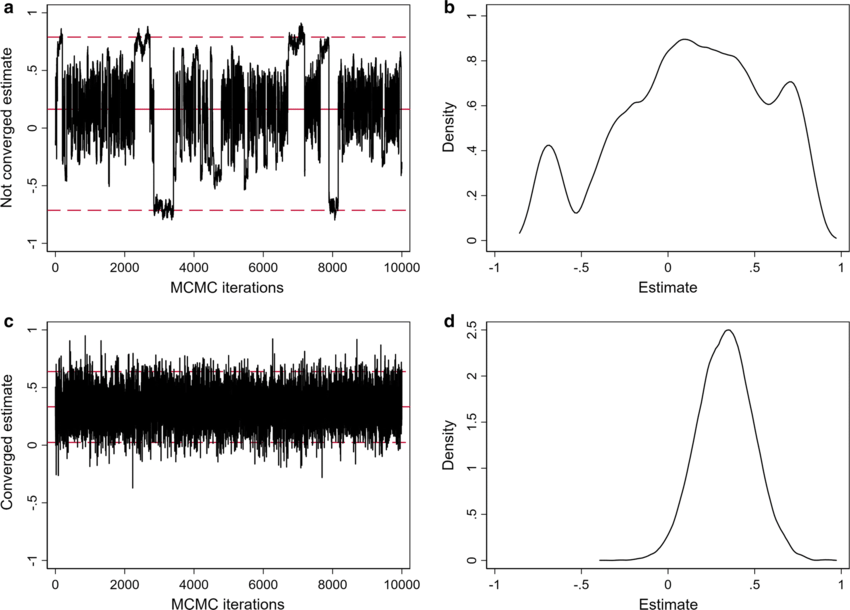
\includegraphics[scale=0.25]{figures/traceplots.png}
\end{figure}
\begin{idea}[No one diagnostic is enough]
 Use multiple diagnostic metrics, always.
 Every MCMC diagnostic out there has blind spots; using multiple simultaneously increases the chances those blind spots are covered.
\end{idea}
\end{frame}
%%%%%%%%%%%%%%%%%%%%%%%%%%%%%%%%%%%
\begin{frame}{Scaling with dimension}
\begin{figure}
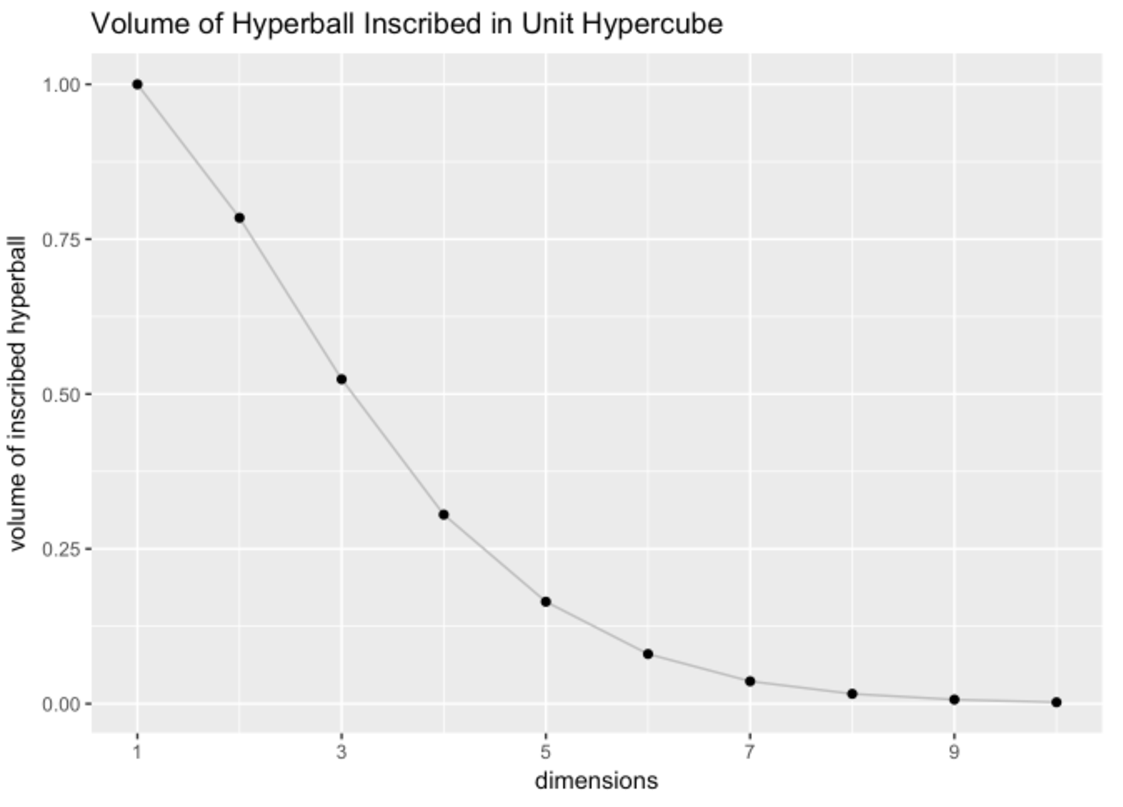
\includegraphics[scale=0.35]{figures/concentration_measure_volume.pdf}
\end{figure}
Taken from~\url{https://mc-stan.org/users/documentation/case-studies/curse-dims.html}.
\begin{idea}[The higher the dimension, the more structure you need]
 As dimension increases, things start to get pretty lonely pretty fast for a particle.
 The only way to counteract this ``thinning'' is to introduce more structure.
 This is the intuitive basis for the success of gradient-based methods such as MALA\footnote{Metropolis-adjusted Langevin algorithm} and HMC\footnote{Hamiltonian (or Hybrid) Monte Carlo.}.
\end{idea}
\end{frame}
%%%%%%%%%%%%%%%%%%%%%%%%%%%%%%%%%%%
\begin{frame}{Take home}
\begin{itemize}
 \item MCMC allows us to make inferences about huge models in Science and Engineering;
 \item MCMC is a terrible method, which nevertheless is our best shot at computing high-dimensional integrals;
 \item One has to make sure a CLT holds;
 \item One has to verify diagnostics to ensure no convergence/performance problems are present;
 \item No one diagnostic is enough.
\end{itemize}
\end{frame}
%%%%%%%%%%%%%%%%%%%%%%%%%%%%%%%%%%%
\begin{frame}{Recommended reading}
\begin{itemize}
  \item[\faBook] \cite{Robert2007}, Ch. 6\footnote{The Bayesian Choice by Christian Robert (2007, 2nd edition).}.
  \item[\faBook] \url{https://betanalpha.github.io/assets/case_studies/markov_chain_monte_carlo.html}
 \end{itemize} 
\end{frame}
